\chapter{Implementing the creative system}
\label{ch:implementation}

% OK

This chapter goes over the technical details of the implementation of the system.
Firstly, the used pre-trained StyleGAN2 model \citep{stylegan2} is discussed. 
The issues with and extensions made to the GANSpace tool \citep{ganspace} are also explained here.
Since the GANSpace tool lacks documentation and support, special attention has been taken to ensure reproducibility.

%------------------------------------
\section{Using StyleGAN2 model}
\label{sec:sytelgan2_implement}

Using a pre-trained StyleGAN2 model is easy and doesn't require an extraordinary amount of computational power.
As StyleGAN2 is created by researchers at NVidia, it's recommended to have an NVidia GPU, especially one with CUDA support.
These are widely available and the system used for this project had a relatively old GTX 970 with 4 GB of VRAM.
With just a few lines of Python code and the download of a pre-trained model, which is about 1 GB in size, the GAN is loaded in and starts generating images.
The generation of a singular image takes seconds at most for the GTX 970 system.
Google's Colaboratory Notebooks are also capable of doing just this with the free tier.
Since downloading and starting the pre-trained model is taken care of automatically by the extended GANSpace tool, no further instructions are given.

%------------------------------------
\section{Extending the GANSpace tool}
\label{sec:GANSpace_implement}

Whilst GANSpace is an incredibly easy tool to gain interpretable control over a GAN with, it does have some shortcomings and flaws.
As a starter, the documentation isn't up to par and due to the low popularity, troubleshooting isn't an easy task.
The installation guide at the time of writing lacks crucial steps such as specifying all required dependencies and more.
Support for anything other than Linux distributions is poor.
Because of this, it was chosen to create a fresh install of Ubuntu 20.04 and document all steps required to get the tool to work.
These steps and much more documentation are available on the GitHub repository of this project \citep{github_project}.
The new setup guide is available under the GANSpace folder as SETUP.md, it is also published to the issues page of the GANSpace tool\footnote{\url{https://github.com/harskish/ganspace/issues/49}}. The used Pycuda folder is also made available.

Besides this, a simple script called rungan.sh is made, which upon execution initializes the GANSpace environment exactly as it was used for this paper.
After successfully running this script, a screen as shown in figure \ref{fig:extended_ganspace_tool} should be presented.
Note the visual queues such as the setting field being set to 'Creative Car Design' and the title of the window being custom for the project.
The most important added feature is the possibility of saving the canvas.
This works for all possible batch sizes.
The code responsible for generating different images after resampling the latent space is also discussed inside the exploring\_GANSpace.md file under the GANSpace folder.
This is important for the similarity measure as is discussed in the evaluation chapter of this paper.


\begin{figure*}
\centering
\begin{subfigure}{.5\textwidth}
  \centering
  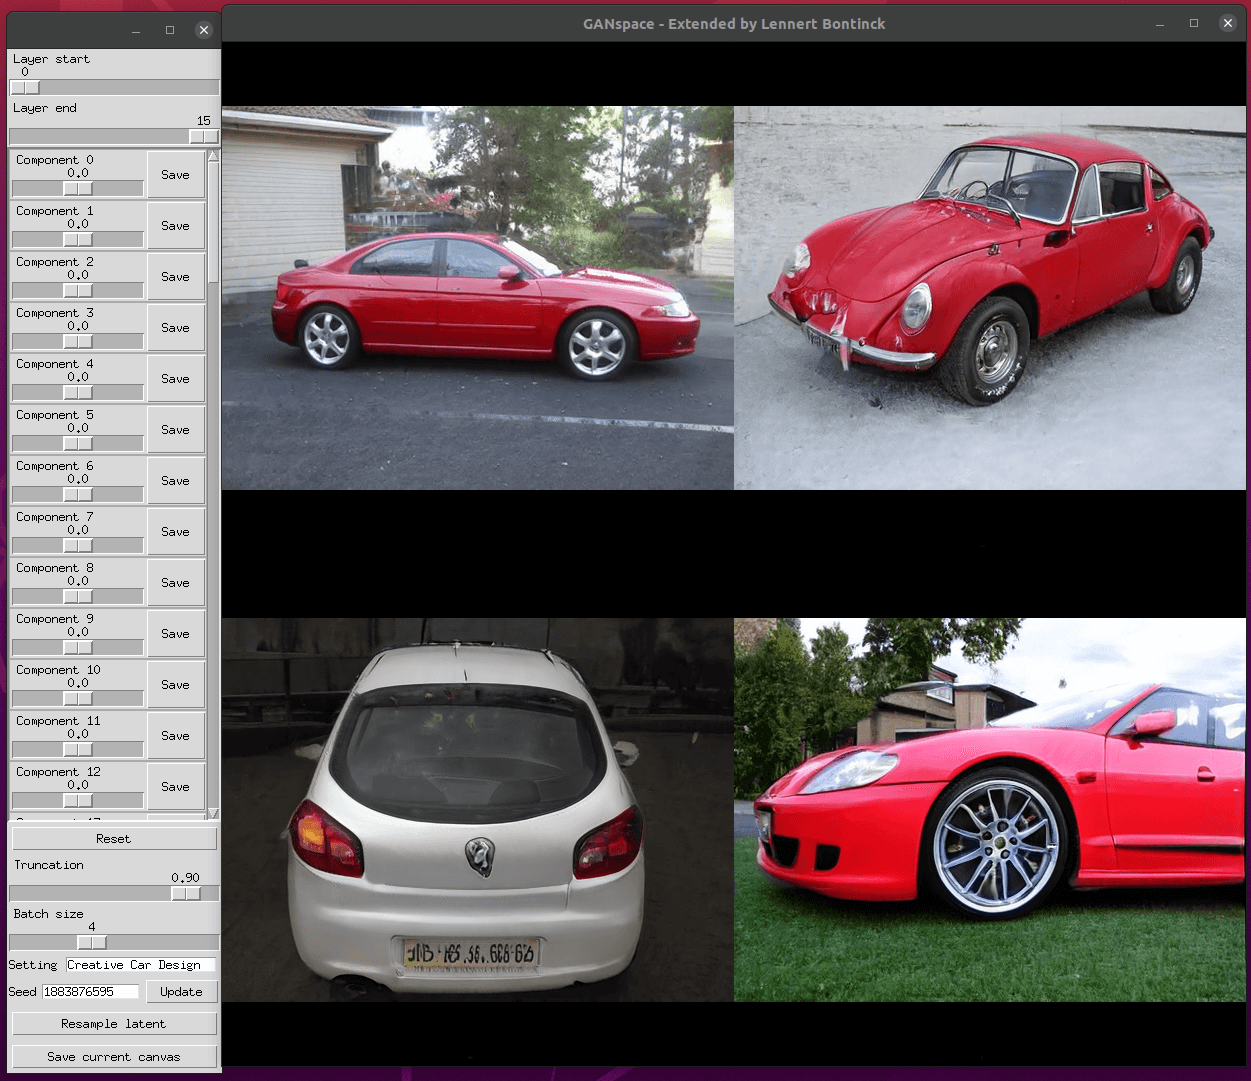
\includegraphics[width=\textwidth]{images/extended_ganspace.png}
  \caption{Extended GANSpace tool}
  \label{fig:extended_ganspace_tool}
\end{subfigure}%
\hspace{1cm}
\begin{subfigure}{.4\textwidth}
  \centering
  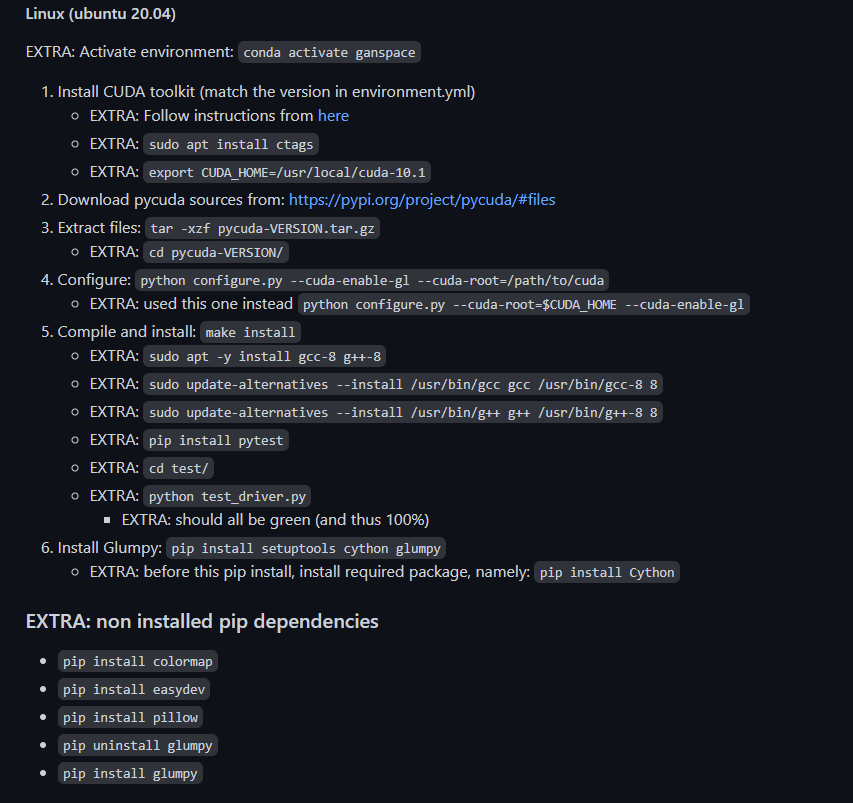
\includegraphics[width=\textwidth]{images/documentation.PNG}
  \caption{Exhaustive documentation}
  \label{fig:extended_ganspace_doc}
\end{subfigure}
\captionsetup{width=.85\linewidth}
\caption{Screenshot of the extended GANSpace tool and documentation.}
\label{fig:extended_ganspace}
\end{figure*}


%------------------------------------
\section{Reproducibility}
\label{sec:reproducibility_implement}

In contrast with the original GANSpace tool documentation, this project contains all required details on downloading and running all required dependencies and code.
The custom made script that was discussed allows for a one-line command to initialize the GANSpace tool identically to the one used.
It downloads the discussed pre-trained StyleGAN2 model automatically. 
All of the settings for generated images and found modifications are also written down.
These are documented in the exploring\_GANSpace.md file under the GANSpace folder as well as the README.md of the generated images folder.
This means that by simply setting the seed and changing the corresponding sliders as documented, identical results can be achieved.